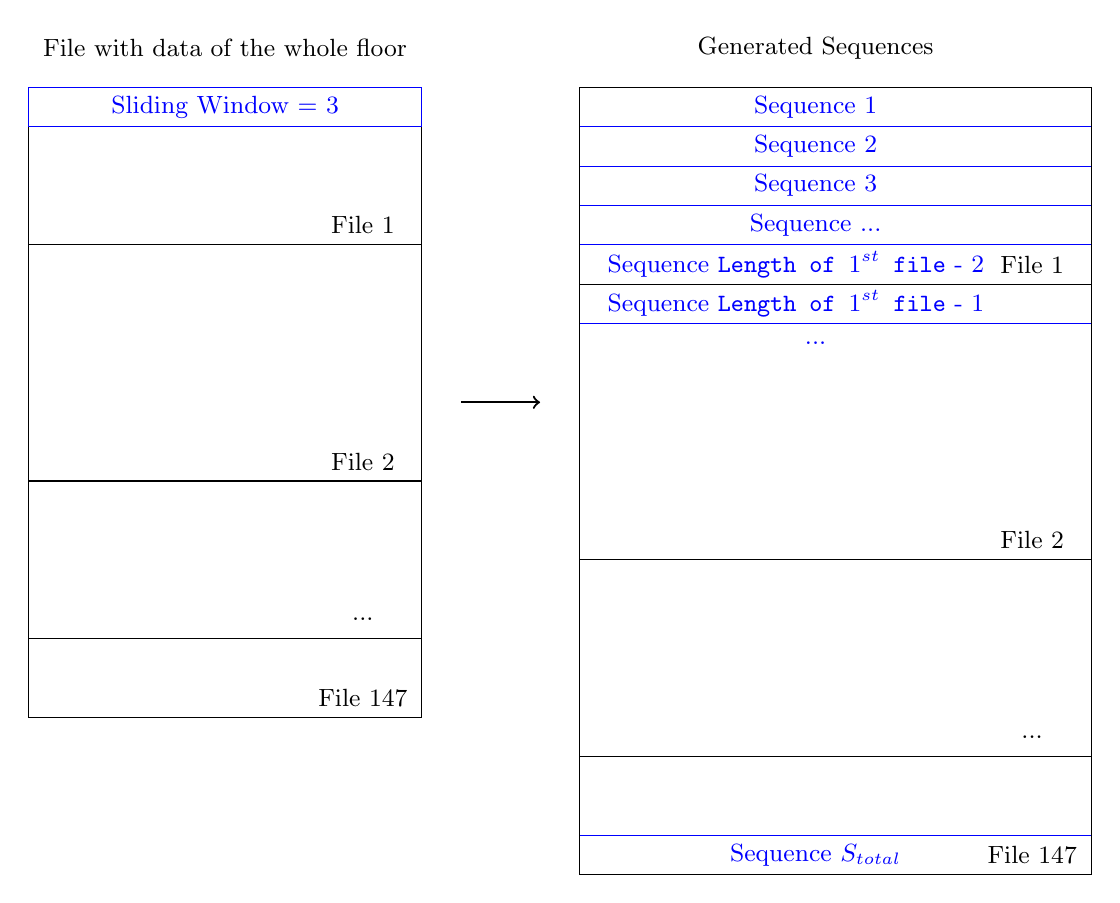
\begin{tikzpicture}

% File representation
\draw[black] (1,1) rectangle (6,9);
\draw[black] (1,7) -- (6,7);
\node[align=center, black, font=\small] at (5.25, 7.25) {File 1};
\draw[black] (1,4) -- (6,4);
\node[align=center, black, font=\small] at (5.25, 4.25) {File 2};
\draw[black] (1,2) -- (6,2);
\node[align=center, black, font=\small] at (5.25, 2.25) {...};
\node[align=center, black, font=\small] at (5.25, 1.25) {File 147};
\node[align=center, font=\small] at (3.5, 9.5) {File with data of the whole floor};

% Sliding window representation
\draw[blue] (1,8.5) rectangle (6,9);
\node[align=center, blue, font=\small] at (3.5, 8.75) {Sliding Window = 3};

% Arrow
\draw[->, thick] (6.5,5) -- (7.5,5);

% Generated sequences representation
\draw[blue] (8,8.5) rectangle (14.5,9);
\node[align=center, blue, font=\small] at (11, 8.75) {Sequence 1};
\draw[blue] (8,8) rectangle (14.5,8);
\node[align=center, blue, font=\small] at (11, 8.25) {Sequence 2};
\draw[blue] (8,7.5) rectangle (14.5,8);
\node[align=center, blue, font=\small] at (11, 7.75) {Sequence 3};
\draw[blue] (8,7) rectangle (14.5,7.5);
\node[align=center, blue, font=\small] at (11, 7.25) {Sequence ...};
\draw[blue] (8,6.5) rectangle (14.5,7);
\node[align=center, blue, font=\small] at (10.75, 6.75) {Sequence \texttt{Length of $1^{st}$ file} - 2};
\draw[blue] (8,6) rectangle (14.5,6.5);
\node[align=center, blue, font=\small] at (10.75, 6.25) {Sequence \texttt{Length of $1^{st}$ file} - 1};
\draw[blue] (8,-.5) rectangle (14.5,6);
\node[align=center, blue, font=\small] at (11, 5.75) {...};
\draw[blue] (8,-1) rectangle (14.5,-.5);
\node[align=center, blue, font=\small] at (11, -.75) {Sequence $S_{total}$};

\draw[black] (8,-1) rectangle (14.5,9);
\draw[black] (8,6.5) -- (14.5,6.5);
\node[align=center, black, font=\small] at (13.75, 6.75) {File 1};
\draw[black] (8,3) -- (14.5,3);
\node[align=center, black, font=\small] at (13.75, 3.25) {File 2};
\draw[black] (8,.5) -- (14.5,.5);
\node[align=center, black, font=\small] at (13.75, .75) {...};
\node[align=center, black, font=\small] at (13.75, -.75) {File 147};
\node[align=center, black, font=\small] at (11, 9.5) {Generated Sequences};

\end{tikzpicture}
    